\documentclass{article}
\usepackage[utf8]{inputenc}
\usepackage[T2A]{fontenc}
\usepackage[utf8]{inputenc}
\usepackage[russian]{babel}
\usepackage[pdftex]{graphicx}
\graphicspath{ {./zxc/} }
\title{ТВМ ДЗ1}
\author{Alexsander Singin}
\date{04.04.2022}

\begin{document}

\maketitle
\clearpage	                    
\section{Задание 1. Построить конечный автомат, распознающий язык}
  1. L = $\{w \in \{a,b,c\}*| |w|_c = 1\} $\\
  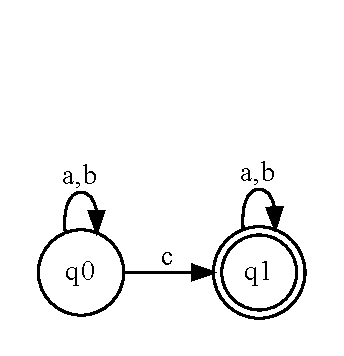
\includegraphics[scale = 1]{zxc/1.1.pdf}\\
  2. L = $\{w \in \{a,b\} * | |w|_a \leq 2, |w|_b \geq 2 \}$\\
  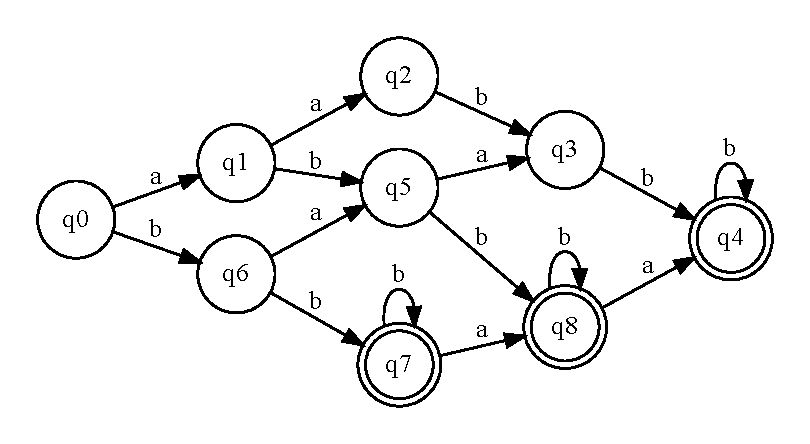
\includegraphics[scale = 1]{zxc/1.2.pdf}\\
  3. L = $\{w \in \{a,b\} * | |w|_a \neq |w|_b \} $\\
  Язык $\bar L$ не является регулярным, что мы выяснеем по лемме о разрастании, следовательно язык L тоже не является регулярным\\
  4. L = $\{w \in \{a,b\} * |ww = www \} $\\
  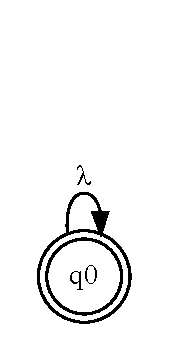
\includegraphics[scale = 1]{zxc/1.4.pdf}\\
  \section{Задание 2. Построить конечный автомат, используя прямо произведение}\\
  1. $L_1 = \{w \in \{a,b\} | |w|_a \geq 2 \wedge |w|_b \geq 2 \} $\\
  $L_{11} = \{w \in \{a,b\} | |w|_a \geq 2$\\
  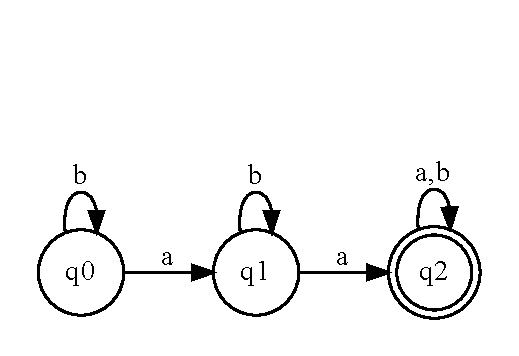
\includegraphics[scale = 1]{zxc/2.1.pdf}\\
  $L_{12} = \{w \in \{a,b\} | |w|_b \geq 2$\\
  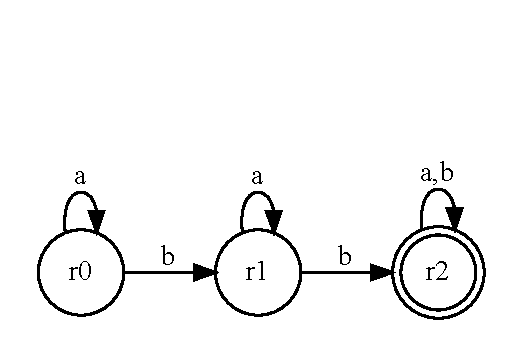
\includegraphics[scale = 1]{zxc/2.2.pdf}\\
  Далее найдем прямое произведение $L_{11}$ и $L_{12}$ = \\
  $L_{11}\times L_{12}=\langle \sum_L_{11}\cup\sum_L_{12}, Q_L_{11}\times Q_L_{12}, \langle s_L_{11},s_L_{12}\rangle, T_L_{11}\times T_L_{12}, \langle\sigma_L_{11}(q_L_{11},c),\sigma_L_{12}(q_L_{12},c) \rangle$
  \begin{itemize}
      \item $\sum - \{a,b\}$\\
      \item Q = $\{q0r0,q0r1,q0r2,q1r0,q1r1,q1r2,q2r0,q2r1,q2r2\}$\\
      \item s = $<s1,s2>$ = q0r0\\
      \item T = $T_1 \times T_2 = q2r2 $\\
      \item $\sigma(<q1,q2>,c> =  < \sigma_1(q1,c),\sigma_2(q2,c)$\\
  \end{itemize}
			\begin{tabular}{ | l | l | l | }
				\hline
				& a & b \\ \hline
				$\langle q_0,r_0\rangle$ & $\langle q_1,r_0\rangle$ & $\langle q_0,r_1\rangle$ \\
				$\langle q_0,r_1\rangle$ & $\langle q_1,r_1\rangle$ & $\langle q_0,r_2\rangle$ \\
				$\langle q_0,r_2\rangle$ & $\langle q_1,r_2\rangle$ & $\langle q_0,r_2\rangle$ \\
				$\langle q_1,r_0\rangle$ & $\langle q_2,r_0\rangle$ & $\langle q_1,r_1\rangle$ \\
				$\langle q_1,r_1\rangle$ & $\langle q_2,r_1\rangle$ & $\langle q_1,r_2\rangle$ \\
				$\langle q_1,r_2\rangle$ & $\langle q_2,r_2\rangle$ & $\langle q_1,r_1\rangle$ \\
				$\langle q_2,r_0\rangle$ & $\langle q_2,r_0\rangle$ & $\langle q_2,r_1\rangle$ \\
				$\langle q_1,r_1\rangle$ & $\langle q_2,r_1\rangle$ & $\langle q_2,r_2\rangle$ \\
				$\langle q_1,r_2\rangle$ & $\langle q_2,r_2\rangle$ & $\langle q_2,r_2\rangle$ \\
				\hline
			\end{tabular}\\
  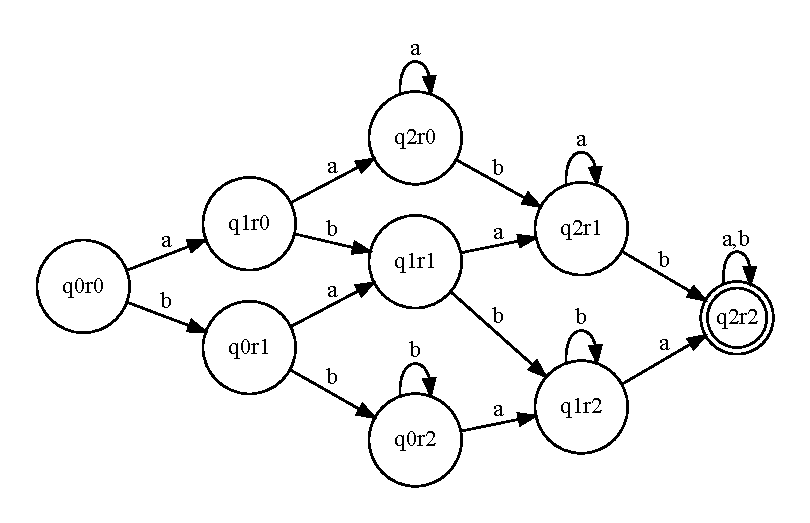
\includegraphics[scale = 1]{zxc/2.3.pdf}\\
  $2. L_2 = \{w \in \{a,b\} * ||w| \geq 3 \wedge |w|$ нечётное\}\\
  Построим автомат: $L_{11} = \{w \in \{a,b\} * ||w| \geq 3 \}$\\
    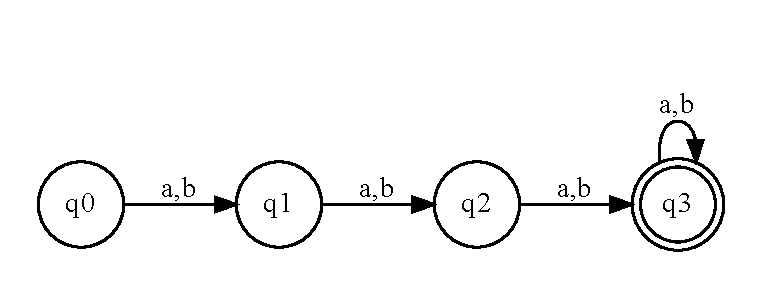
\includegraphics[scale = 1]{zxc/2.4.pdf}\\
  Построим автомат: $L_{12} = \{w \in \{a,b\} * ||w|$ нечётное$\}$ \\
     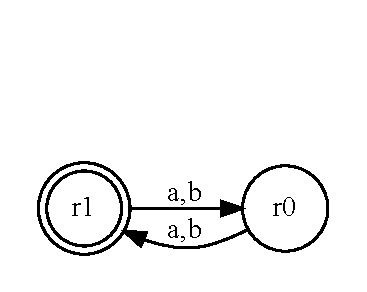
\includegraphics[scale = 1]{zxc/2.5.pdf}\\
    Найдем прямое произведение $L_{11}$ и $l_{12}$ = 
  $L_{11}\times L_{12}=\langle \sum_L_{11}\cup\sum_L_{12}, Q_L_{11}\times Q_L_{12}, \langle s_L_{11},s_L_{12}\rangle, T_L_{11}\times T_L_{12}, \langle\sigma_L_{11}(q_L_{11},c),\sigma_L_{12}(q_L_{12},c) \rangle$
  \begin{itemize}
      \item $\sum - \{a,b\}$\\
      \item Q = $\{q0r0,q0r1,q1r0,q1r1,q2r0,q2r1,q3r0,q3r1\}$\\
      \item s = $<s1,s2>$ = q0r0\\
      \item T = $T_1 \times T_2 = q3r1 $\\
      \item $\sigma(<q1,q2>,c> =  < \sigma_1(q1,c),\sigma_2(q2,c)$\\
  \end{itemize}
			\begin{tabular}{ | l | l | l | }
				\hline
				& a & b \\ \hline
				$\langle q_0,r_0\rangle$ & $\langle q_1,r_1\rangle$ & $\langle q_1,r_1\rangle$ \\
				$\langle q_0,r_1\rangle$ & $\langle q_1,r_0\rangle$ & $\langle q_1,r_0\rangle$ \\
				$\langle q_1,r_0\rangle$ & $\langle q_2,r_1\rangle$ & $\langle q_2,r_1\rangle$ \\
				$\langle q_1,r_1\rangle$ & $\langle q_2,r_0\rangle$ & $\langle q_2,r_0\rangle$ \\
				$\langle q_2,r_0\rangle$ & $\langle q_3,r_1\rangle$ & $\langle q_3,r_1\rangle$ \\
				$\langle q_2,r_1\rangle$ & $\langle q_3,r_0\rangle$ & $\langle q_3,r_0\rangle$ \\
				$\langle q_3,r_0\rangle$ & $\langle q_3,r_1\rangle$ & $\langle q_3,r_1\rangle$ \\
				$\langle q_3,r_1\rangle$ & $\langle q_3,r_0\rangle$ & $\langle q_3,r_0\rangle$ \\
				\hline
			\end{tabular}\\
  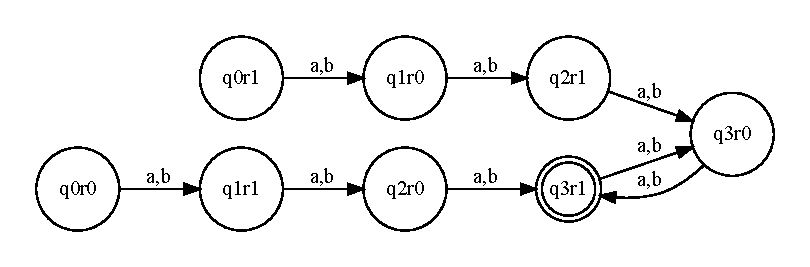
\includegraphics[scale = 1]{zxc/2.6.pdf}\\
    $3. L_3 = \{w \in \{a,b\} * ||w|_a$ четно$ \wedge |w|_b $ кратно трём\}\\
  Построим автомат: $L_{11} = \{w \in \{a,b\} * ||w|_a$ четно$ \}$\\
    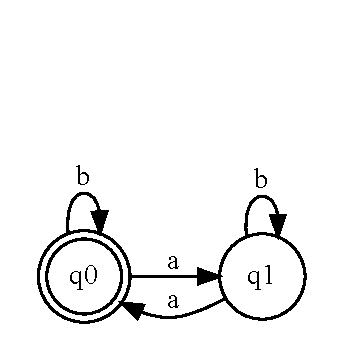
\includegraphics[scale = 1]{zxc/2.7.pdf}\\
  Построим автомат: $L_{12} = \{w \in \{a,b\} * ||w|_b$ кратно трём$\}$ \\
     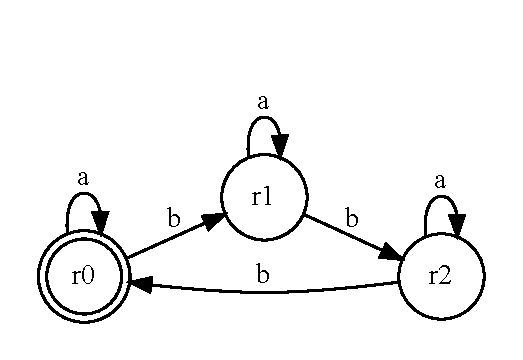
\includegraphics[scale = 1]{zxc/2.8.pdf}\\
    Найдем прямое произведение $L_{11}$ и $l_{12}$ = 
  $L_{11}\times L_{12}=\langle \sum_L_{11}\cup\sum_L_{12}, Q_L_{11}\times Q_L_{12}, \langle s_L_{11},s_L_{12}\rangle, T_L_{11}\times T_L_{12}, \langle\sigma_L_{11}(q_L_{11},c),\sigma_L_{12}(q_L_{12},c) \rangle$
  \begin{itemize}
      \item $\sum - \{a,b\}$\\
      \item Q = $\{q0r0,q0r1,q0r2,q1r0,q1r1,q1r2\}$\\
      \item s = $<s1,s2>$ = q0r0\\
      \item T = $T_1 \times T_2 = q0r0 $\\
      \item $\sigma(<q1,q2>,c> =  < \sigma_1(q1,c),\sigma_2(q2,c)$\\
  \end{itemize}
			\begin{tabular}{ | l | l | l | }
				\hline
				& a & b \\ \hline
				$\langle q_0,r_0\rangle$ & $\langle q_1,r_0\rangle$ & $\langle q_0,r_1\rangle$ \\
				$\langle q_0,r_1\rangle$ & $\langle q_1,r_1\rangle$ & $\langle q_0,r_2\rangle$ \\
				$\langle q_0,r_2\rangle$ & $\langle q_2,r_2\rangle$ & $\langle q_0,r_0\rangle$ \\
				$\langle q_1,r_0\rangle$ & $\langle q_0,r_0\rangle$ & $\langle q_1,r_1\rangle$ \\
				$\langle q_1,r_1\rangle$ & $\langle q_0,r_1\rangle$ & $\langle q_1,r_2\rangle$ \\
				$\langle q_1,r_2\rangle$ & $\langle q_0,r_2\rangle$ & $\langle q_1,r_0\rangle$ \\
				\hline
			\end{tabular}\\
  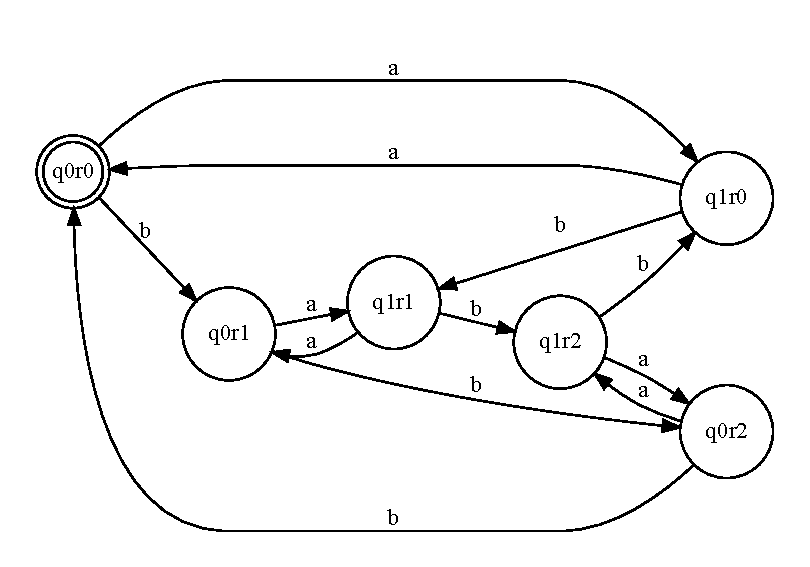
\includegraphics[scale = 1]{zxc/2.9.pdf}\\
  4. $L_4 = \bar L_3$\\
    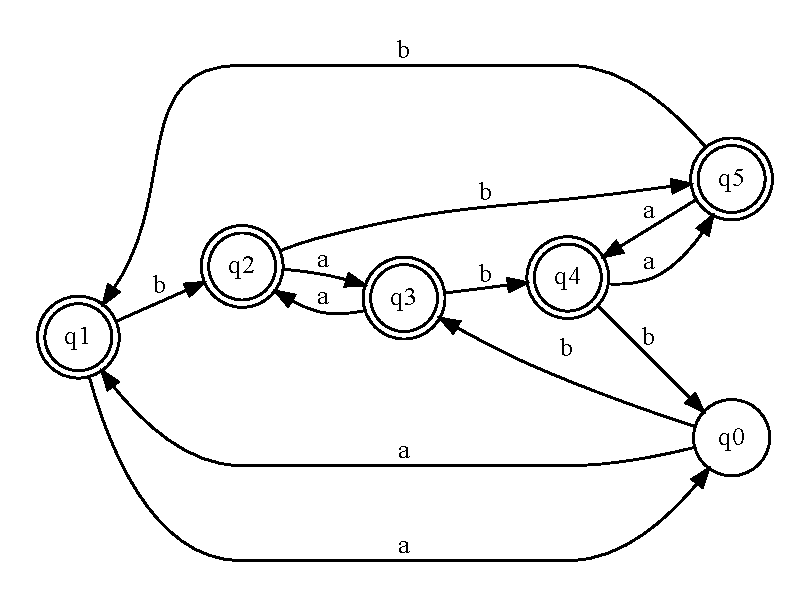
\includegraphics[scale = 1]{zxc/2.10.pdf}\\
  5. $L_5 = L_2\setminus L_3 = L_2\cap \bar L_3$
  $L_{11}$:\\
    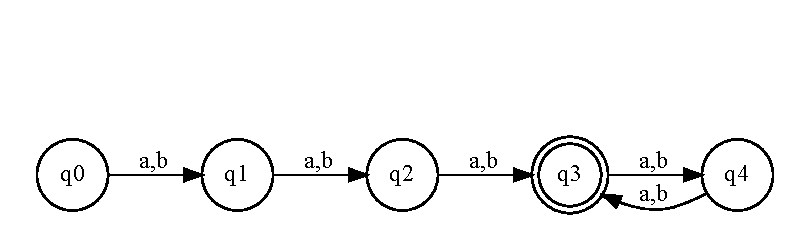
\includegraphics[scale = 1]{zxc/2.11.pdf}\\
    $L_{12}$:\\
      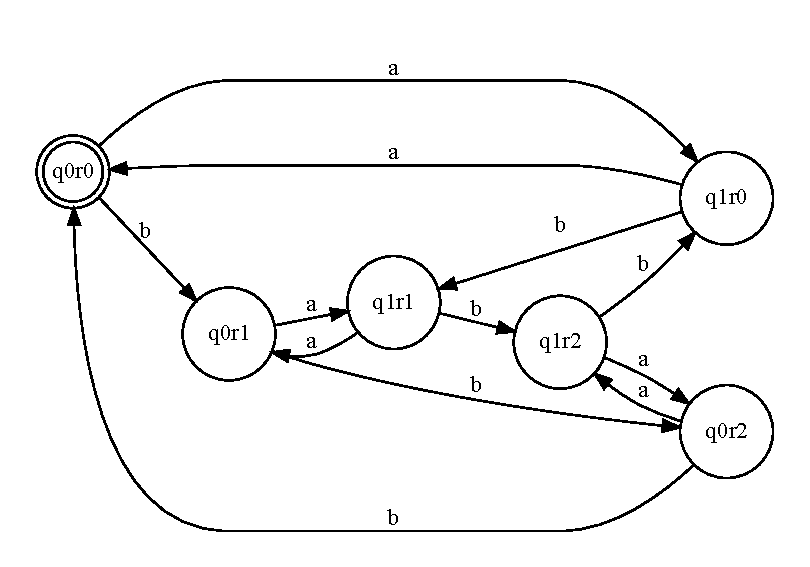
\includegraphics[scale = 1]{zxc/2.9.pdf}\\
  \begin{itemize}
      \item $\sum - \{a,b\}$\\
      \item Q = $\{q0r0,q0r1,q0r2,q0r3,q0r4,q0r5,q1r0,q1r1,q1r2,q1r3,q1r4,q1r5,q2r0,q2r1,q2r2,q2r3,q2r4,q2r5,q3r0,q3r1,q3r2,q3r3,q3r4,q3r5,q4r0,q4r1,q4r2,q4r3,q4r4,q4r5\}$\\
      \item s = $<s1,s2>$ = q1r1\\
      \item T = $T_1 \times T_2 = q3r1,q3r2,q3r3,q3r4,q3r5 $\\
      \item $\sigma(<q1,q2>,c> =  < \sigma_1(q1,c),\sigma_2(q2,c)$\\
  \end{itemize}
			\begin{tabular}{ | l | l | l | }
				\hline
				& a & b \\ \hline
				$\langle q_0,r_0\rangle$ & $\langle q_1,r_1\rangle$ & $\langle q_1,r_3\rangle$ \\
				$\langle q_1,r_1\rangle$ & $\langle q_2,r_0\rangle$ & $\langle q_2,r_2\rangle$ \\
				$\langle q_1,r_3\rangle$ & $\langle q_2,r_2\rangle$ & $\langle q_2,r_4\rangle$ \\
				$\langle q_2,r_0\rangle$ & $\langle q_3,r_1\rangle$ & $\langle q_3,r_3\rangle$ \\
				$\langle q_2,r_2\rangle$ & $\langle q_3,r_3\rangle$ & $\langle q_3,r_4\rangle$ \\
				$\langle q_2,r_4\rangle$ & $\langle q_3,r_5\rangle$ & $\langle q_3,r_0\rangle$ \\
				$\langle q_3,r_0\rangle$ & $\langle q_4,r_1\rangle$ & $\langle q_4,r_3\rangle$ \\
				$\langle q_3,r_1\rangle$ & $\langle q_4,r_0\rangle$ & $\langle q_4,r_2\rangle$ \\
				$\langle q_3,r_2\rangle$ & $\langle q_4,r_3\rangle$ & $\langle q_4,r_5\rangle$ \\
				$\langle q_3,r_3\rangle$ & $\langle q_4,r_2\rangle$ & $\langle q_4,r_4\rangle$ \\
				$\langle q_3,r_4\rangle$ & $\langle q_4,r_5\rangle$ & $\langle q_4,r_0\rangle$ \\
				$\langle q_3,r_5\rangle$ & $\langle q_4,r_4\rangle$ & $\langle q_4,r_1\rangle$ \\
				$\langle q_4,r_0\rangle$ & $\langle q_5,r_1\rangle$ & $\langle q_3,r_3\rangle$ \\
				$\langle q_4,r_1\rangle$ & $\langle q_5,r_0\rangle$ & $\langle q_3,r_2\rangle$ \\
				$\langle q_4,r_2\rangle$ & $\langle q_5,r_3\rangle$ & $\langle q_3,r_5\rangle$ \\
				$\langle q_4,r_3\rangle$ & $\langle q_5,r_2\rangle$ & $\langle q_3,r_4\rangle$ \\
				$\langle q_4,r_4\rangle$ & $\langle q_5,r_5\rangle$ & $\langle q_3,r_0\rangle$ \\
				$\langle q_4,r_5\rangle$ & $\langle q_5,r_4\rangle$ & $\langle q_3,r_1\rangle$ \\
				\hline
			\end{tabular}\\
    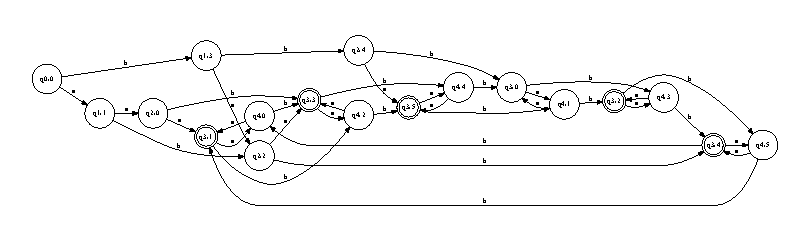
\includegraphics[scale = 1.2]{zxc/2.12.pdf}\\
\section{3.Построить минимальный ДКА по выражению}
1.{\large\item $(ab+aba)^*a$} \\
Строим НКА:\\
    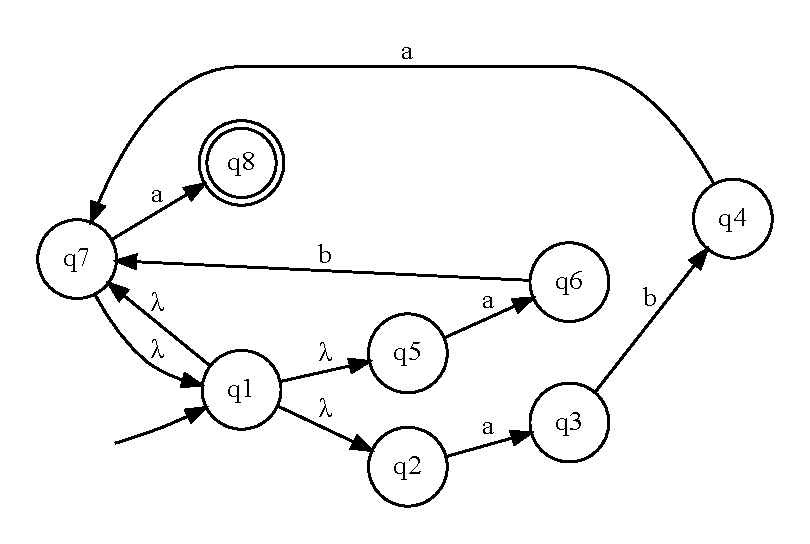
\includegraphics[scale = 1.0]{zxc/3.1.pdf}\\
Строим минимизированный ДКА:\\
    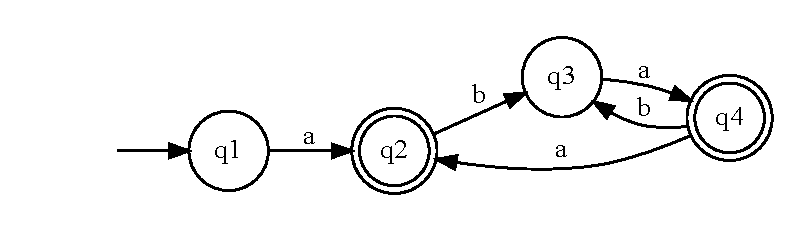
\includegraphics[scale = 1.0]{zxc/3.2.pdf}\\
2.{\large\item $a(a(ab)^*b)^*(ab)^*$} \\
Строим НКА:\\
    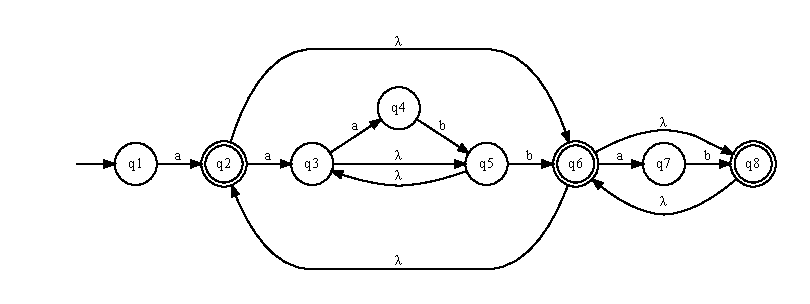
\includegraphics[scale = 1.0]{zxc/3.3.pdf}\\
Строим минимизированный ДКА:\\
    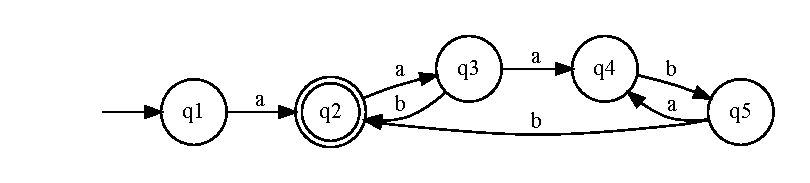
\includegraphics[scale = 1.0]{zxc/3.4.pdf}\\
3.{\large\item $(a+(a+b)(a+b)b)^*$} \\
Строим НКА:\\
    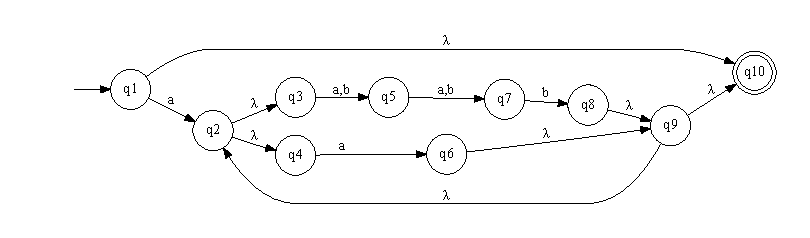
\includegraphics[scale = 1.0]{zxc/3.5.pdf}\\
Строим минимизированный ДКА:\\
    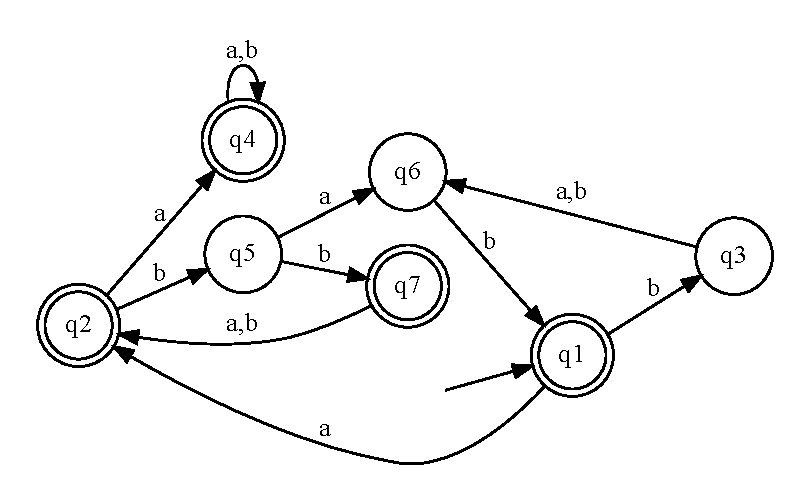
\includegraphics[scale = 1.0]{zxc/3.6.pdf}\\
4.{\large\item $(b+c)((ab)^*c+(ba)^*)^*$} \\
Строим НКА:\\
    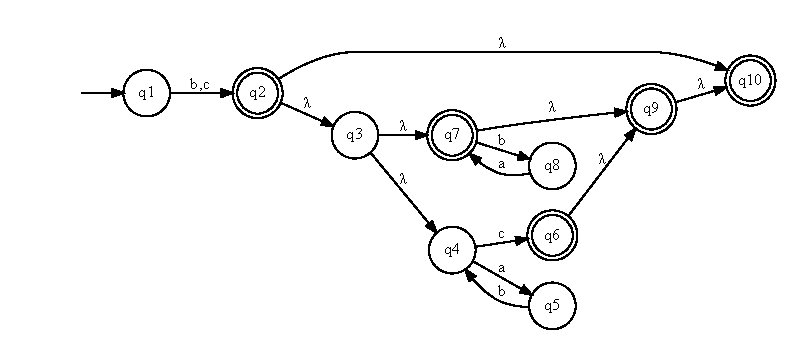
\includegraphics[scale = 1.0]{zxc/3.7.pdf}\\
Строим минимизированный ДКА:\\
    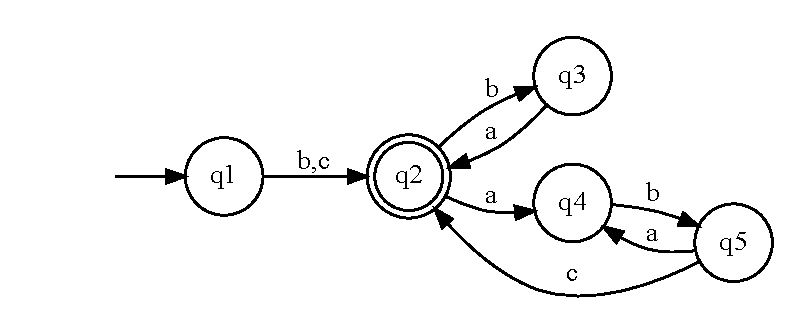
\includegraphics[scale = 1.0]{zxc/3.8.pdf}\\
5.{\large\item $(a+b)^+(aa+bb+abab+baba)(a+b)^+$} \\
Строим НКА:\\
    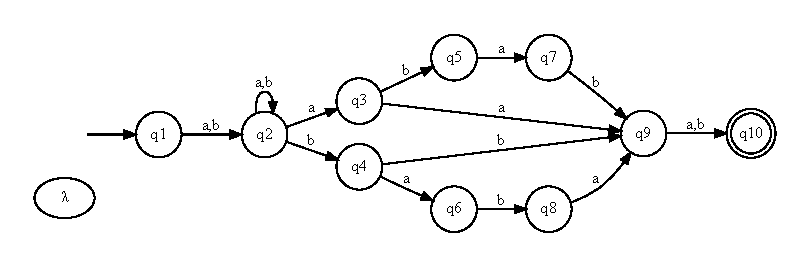
\includegraphics[scale = 1.0]{zxc/3.9.pdf}\\
Строим минимизированный ДКА:\\
    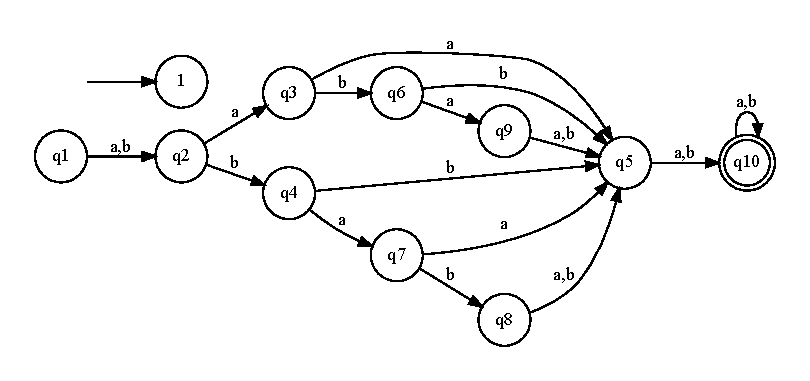
\includegraphics[scale = 1.0]{zxc/3.10.pdf}\\
\section{4.Определить, является ли данный язык регулярным}\\
4.1 ${\large\item L=\{uaav\ |\ u\in\{a,b\}^*,v\in\{a,b\}^*, |u|_b\geq |v|_a \}}$ \\
Язык является регулярным, так как существует автомат распознающий его
    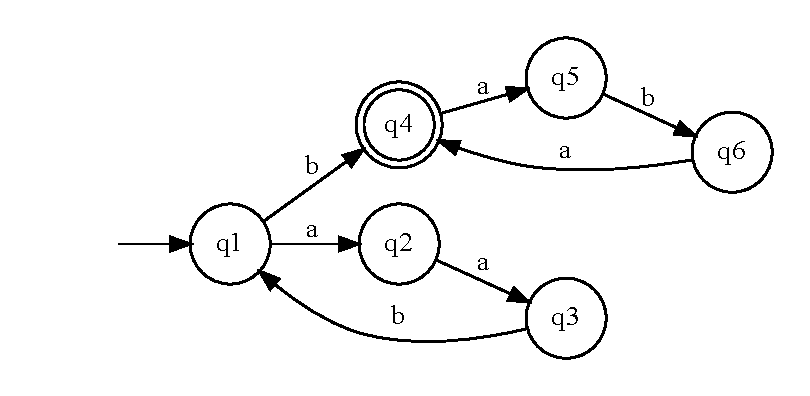
\includegraphics[scale = 1.0]{zxc/4.1.pdf}\\
4.2 {\large\item $L=\{uaav\ |\ u\in\{a,b\}^*,v\in\{a,b\}^*, |u|_b\geq |v|_a \}$} \\
	$\forall n=N \omega:\omega=b^{N+1}aaa^{N+1}, \in L, |\omega|=2N+4 $, из леммы о разрастании мы знаем, что $|xy|\leq N,следовательно;$ для любого произвольного $x , y,\ y=b^i$, что означет то, что $xy^kz$ выходит за пределы языка при k=0 из чего следует, что язык L не регулярный\\
4.3 {\large\item $L=\{a^m\omega\ |\ \omega\in\{a,b\}^*, 1\leq |\omega| \leq m \}$} \\\\
	 $\forall n=N$  $\alpha:a^{N+1}ba^{N},\ \alpha \in L, |\omega|=N+1 $, из леммы о разрастании  $|xy|\leq N,$ для любого произвольного $x , y,\ y=a^i;$ следует, что $xy^kz$ выходит за пределы языка при k=0,та как при |\alpha|>количества букв a слева, следовательно $ язык L не регулярный\\
4.4 {\large\item $L=\{a^kb^ma^n\ |\ k=n\ \lor \ m>0 \}$} \\
Язык является регулярным, так как существует автомат распознающий его\\
    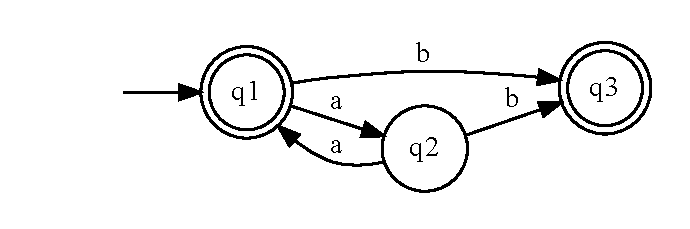
\includegraphics[scale = 1.0]{zxc/4.4.pdf}\\
4.5 	{\large\item $L=\{ucv\ |\ u\in\{a,b\}^*, v\in\{a,b\}^*, u\neq v^R \}$} \\
	Рассмотрим $\bar{L}$. $\bar{L}=\{ucv\ |\ u\in\{a,b\}^*, v\in\{a,b\}^*, u=v^R \}$\\
	$\forall n \omega:\omega=b^ncb^n, \in \bar{L}, |\omega|=2n+1 $, из леммы о рарастании мы знаем, что $|xy|\leq n,$ при любых значениях x,y $x , y,\ y=b^i \implies xy^kz$ выходит за пределы языка при k>1 язык $\bar{L}$ не регулярный, следовательно язык $L$ не регулярный\\
\end{document}